\documentclass[12pt]{article}
\usepackage[utf8]{inputenc}
\usepackage{amsmath}
\usepackage{hyperref}
\usepackage{graphicx}
\usepackage[swedish]{babel}
\title{Andragradsfunktioner}
\date{}
\begin{document}
  \maketitle
  
  
  
  \section{Introduktion}
  Det här dokumentet kommer från en fritt tillgänglig text på webbplatsen GitHub (se \url{https://github.com/Itangalo/Andragradsfunktioner}).
  Alla som är intresserade är inbjudna att föreslå och diskutera ändringar och förbättringar.
  Det kan man antingen göra genom att starta diskussioner i projektets ``issue queue'' (alternativt kommentera i befintliga diskussioner), eller genom att göra en kopia (``klon'') av hela projektet och redigera så mycket man vill.
  Om man är nöjd med sina ändringar, och vill att de ska tas in i ursprungliga dokumentet, kan man markera detta -- så kan förslaget diskuteras av andra inblandade.

  Innehållet i det här projektet är tillgänglig under Creative Commons-licens \href{http://creativecommons.org/licenses/by-nc-sa/3.0/}{attribution+non-commercial+share alike}.


  \section{Första skisser}
  
  (Det här är bara första skisser på upplägg av innehåll i dokumentet.)

  \subsection{Översikt av egenskaper för andragradsfunktioner.}
  Andragradsfunktioner har en högsta eller lägsta punkt, vilket gör dem användbara för att modellera vissa typer av samband.
  (Utgångspunkt i sådana samband!)
  Vad extrempunkt och extremvärde betyder, och varför de är viktiga begrepp i tillämpad matematik.

  \subsection{Hur uttrycket $f(x) = a(x+d)^2+e$ beter sig}
  Det finns olika sätt att representera andragradsuttryck, och $a(x+d)^2+e$ är en form som är praktisk för att se engenskaper hos funktioner.
  Utforskande av hur de olika parametrarna påverkar funktionens graf, framförallt hur $d$ och $e$ hänger samman med extrempunkt/extremvärde.
  (Bifogad GeoGebra-demonstration!)
  Fördjupning: Parametrarna $d$ och $e$, och translation av funktioner.
  
  \subsection{Andragradsekvationer}
  Motivering av ekvationer av typen $a(x+d)^2+e=k$.
  Hur man löser sådana ekvationer, med utgångspunkt i potensekvationen $x^2 = k$.
  Fördjupning: Jämförelse med substitutionen $t=x+d$.

  \subsection{Kvadratkomplettering med ansättning}
  Introduktion av andragradsuttryck på formen $ax^2+bx+c$, och hur parametern $c$ avspeglas i funktionens graf.
  Resonemang kring att det finns något uttryck $a(x+d)^2+e$ som representerar varje uttryck på formen $ax^2+bx+c$.
  Kvadreringsregler: utveckla uttryck på formen $(a+b)^2$ eller $(a-b)^2$.
  (Inklusive länk till digital mängdträning, som även omfattar andra parentesmultiplikationer.)
  Hur man kan översätta formen $ax^2+bx+c$ till kvadratkompletterad form (genom ansättning).
  Fördjupning: Vad ansättning egentligen innebär.
  
  \subsection{Överblivet}
  \begin{itemize}
    \item Faktorisering som genväg för att lösa andragradsekvationer
    \item Konjugatregeln. (Ha tillsammans med kvadreringsreglerna?)
    \item Komplexa tal och komplexa lösningar till andragradsekvationer
    \item Hur man kan hitta parametrarna $a$/$d$/$e$ eller $a$/$b$/$c$ från givna punkter
    \item Symmetrilinje för andragradsfunktioner
  \end{itemize}
  
  \begin{figure}
  \centering
  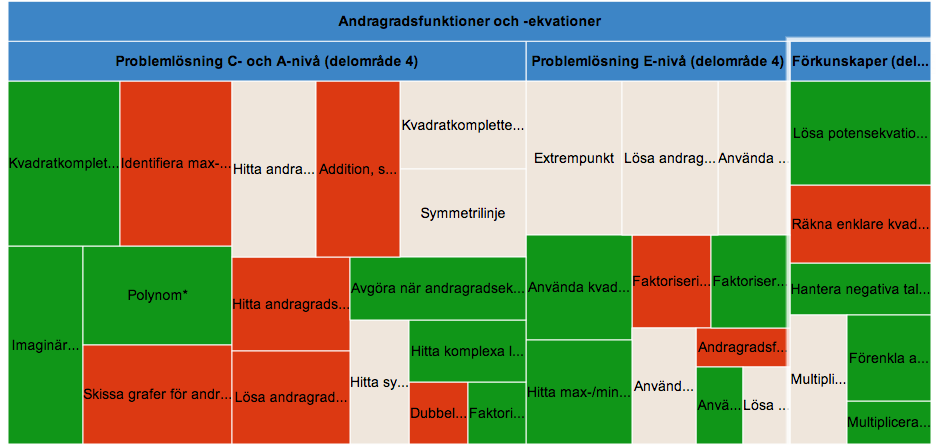
\includegraphics[width=0.3\textwidth]{bilder/testbild.png}
  \caption{\label{fig:testbild}Det här är bara ett test, för att se hur det fungerar att bädda in bilder.}
  \end{figure}

  \section{Varför andragradsfunktioner?}

Tidigare i kursen har vi tittat på linjära funktioner.
De är användbara i många olika sammanhang, inte minst för att skapa modeller för hur olika saker hänger samman:
hur fattigdom påverkar livslängd i ett land, hur koldioxidutsläpp påverkar globala medeltemperaturen, hur pluggtid påverkar hur man lyckas i skolan, med mera.

Men det finns också samband där det \emph{inte} är lyckat att använda räta linjer för att skapa modeller.
Här är ett exempel.

\begin{figure}
  \centering
  \includegraphics[width=0.3\textwidth]{bilder/bensinforbrukning.png}
  \caption{\label{fig:bensinförbrukning}Bensinförbrukning vid olika hastigheter (för en viss bilmodell).}
\end{figure}

Diagrammet visar hur bensinförbrukningen för en viss bilmodell påverkas av hur fort man kör.
Förbrukningen ökar eller minskar inte med någon jämn takt -- istället verkar den visa att det finns en lägsta bensinförbrukning om man kör ca 60--80 km/h.
Om vi försökte beskriva det här sambandet med en rät linje skulle vi helt missa att det finns en bästa hastighet att hålla, eftersom en rät linje skulle visa att bensinförbrukningen hela tiden ökar (eller minskar, beroende på lutning).

Här är ett annat exempel.

\begin{figure}
  \centering
  \includegraphics[width=0.3\textwidth]{bilder/biljettpriser.png}
  \caption{\label{fig:biljettpriser}Total vinst vid olika priser på bussbiljetter.}
\end{figure}

Det här diagrammet visar (ett påhittat) försök med olika biljettpriser på bussen, i en svensk stad.
Med höga priser gör bussbolaget mycket vinst per biljett, men samtidigt är det få personer som köper biljetter.
Med låga priser är det många som väljer att åka buss, men vinsten för varje biljett blir mindre.
Någonstans i mitten ligger det ``bästa'' biljettpriset (åtminstone om målet är att maximera vinsten).

\subsection {Andragradsfunktioner och extrempunkter}

För att modellera samband som har en högsta eller lägsta punkt använder man ofta något som heter \emph{andragradsfunktioner}.
Att de kallas andragradsfunktioner beror på att de innehåller en term med $x^2$ (medan räta linjer skulle kunna kallas förstagradsfunktioner, eftersom de bara innehåller $x^1$).

När vi studerade räta linjen tittade vi särskilt på saker som riktningskoefficient ($k$-värde) och skärning med y-axel ($m$-värde).
För andragradsfunktioner är det andra egenskaper som är intressanta, och den viktigaste av dem är \emph{extrempunkter} eller \emph{extremvärden}.

\begin{itemize}
  \item En \textbf{extrempunkt} är andragradsfunktionens vändpunkt -- det vill säga där funktionen har sitt högsta eller lägsta (mest extrema) värde. (Det är alltså en punkt med både x- och y-värde.)
  \item Ett \textbf{extremvärde} är funktionens värde i extrempunkten. (Det är alltså ett tal.)
  \item Ett \textbf{maximumvärde} är ett extremvärde som är det högsta möjliga, och alltså ligger på en kurva som går upp och sedan ner.
  \item Ett \textbf{minimumvärde} är ett extremvärde som är det lägsta möjliga, och alltså ligger på en kurva som går ned och sedan upp.
  \item En \textbf{parabel} är en graf för en andragradsfunktion.
\end{itemize}

En av de viktigaste användningsområdena för matematik är att hitta extrempunkter för olika samband, vilket inte är så konstigt.
Med hjälp av matematiska analyser kan man få väl underbyggda svar på frågor som:
Hur mycket av kommunbudgeten bör läggas på snöröjning?
Hur mycket ska man träna på gymmet för att få bästa möjliga effekt?
Hur ska vattenreningsverk styras för att dra så lite energi som möjligt?

I många situationer är samband och extrempunkter svåra att hitta, och kräver stora studier.
I det här avsnittet i kursen ska vi titta på några enklare exempel, och se hur vi kan använda andragradsfunktioner för att hitta extrempunkter.



\end{document}
